\documentclass[../../main.tex]{subfiles}

 \lhead{Background}
 
\begin{document}

\section{Background}

	The following section provides the relevant background information that form the basis of the project described in this paper.

%-------------Virtual Acoustic Environments-------------%
	\subsection{Virtual Acoustic Environments}

		 Virtual acoustics has been previously described \cite{Huopaniemi2000} as follows:

		\begin{center}
			\textit{``Virtual acoustics is a general term for the modelling of acoustical phenomena and systems with the aid of a computer''}
		\end{center}

		By this definition, a \ac{VAE} can be thought of as an environment (such as a room) for which the acoustical phenomena have been either recreated or synthesised. To produce a \ac{VAE}, prior knowledge regarding the room which is to be acoustically recreated must be known; how do all audible frequencies propagate around the room for a set sound source location and receiver location?

		This information can be gathered by taking a \ac{RIR} and used to recreate the acoustics of a room for the set sound source and receiver location.

		%  To produce a \ac{VAE}, prior knowledge regarding the sound source, room geometry and listener are required \cite{Huopaniemi2000}.

		%  An example of a \ac{VAE} can be found in previous projects such as \cite{Brereton2012}, upon which this project is based.

		% This essentially means reproducing sounds in an environment other than the one the sound were originally present. However, it can be said that it is possible to produce a \ac{VAE}'s using non-physical methods and could also be rendered through headphones depending on the technique used to capture the 

		% Essentially, \ac{VAE}'s make it sound like someone is in an environment that they're actually not in by producing sound waves that would be present if the they were actually present in that environment. These sound waves can actually be reproduced over headphones as well as loudspeakers, depending on the method used to either capture or synthesise the sound field.

%-------------Room Impulse Responses-------------%
		\subsection{Room Impulse Responses}
			% In order to reproduce the acoustical phenomena of a room, a description of how all audible frequencies interact with that room must be obtained. This can be done by capturing a \ac{RIR}. By placing a sound source and a receiver (microphone) in said room and exciting all audible frequencies, 

			In order to reproduce the acoustical phenomena of a room, an \ac{RIR} must be obtained. This is done by exciting all audible frequencies within the room by using a sound source such as a loudspeaker, and recording the result using a receiver microphone.

			There are a number of techniques used for exciting all audible frequencies. These include an \textbf{impulse} (such as a starter pistol) or an \textbf{exponentially swept sine} for which a sine wave is exponentially increased in frequency over a fixed period of time. Using a starter pistol means that no post processing is required as all the frequencies are excited at the same time and the impulse recorded at the receiver position can be used for convolution with an audio source. Using an exponentially swept sine requires post processing in order to time align all of the frequency dependent room reflections, thus producing an impulse response through the use of a deconvolution algorithm, however this method produces a greater signal to noise ratio thus is the desired method \cite{Stan2002}. 


%-------------Ambisonics-------------%
		\subsection{Ambisonics}

			Ambisonics is a technique used to encode and decode three dimensional spatial audio information using just four audio channels. A sound field can be recorded using a microphone known as a Soundfield microphone. These microphones contain four coincident capsules, one of which is an omni-directional capsule (W) and the rest of which are figure of 8 capsules which are used to record sound in the X (front and back), Y (left and right) and Z (up and down) direction. W channel is used to record the overall sound pressure level and the 

			%-------------Soundfield mic images-------------%
			\begin{figure}[ht]
				\begin{minipage}{0.5\textwidth}
					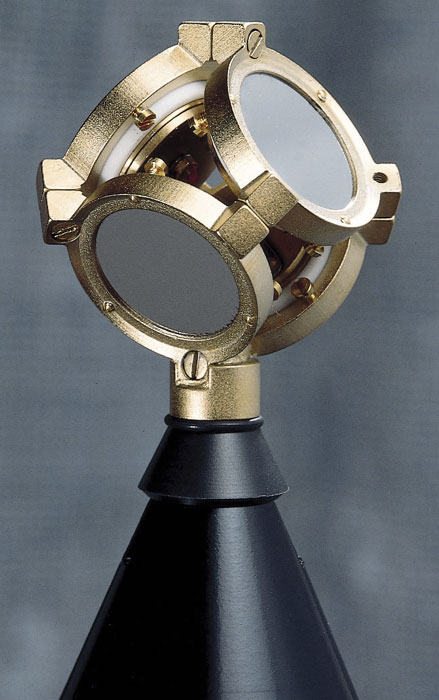
\includegraphics[scale = 0.2]{Sections/Background/images/soudFieldMic.jpg}
				\end{minipage}
				\begin{minipage}{0.5\textwidth}
					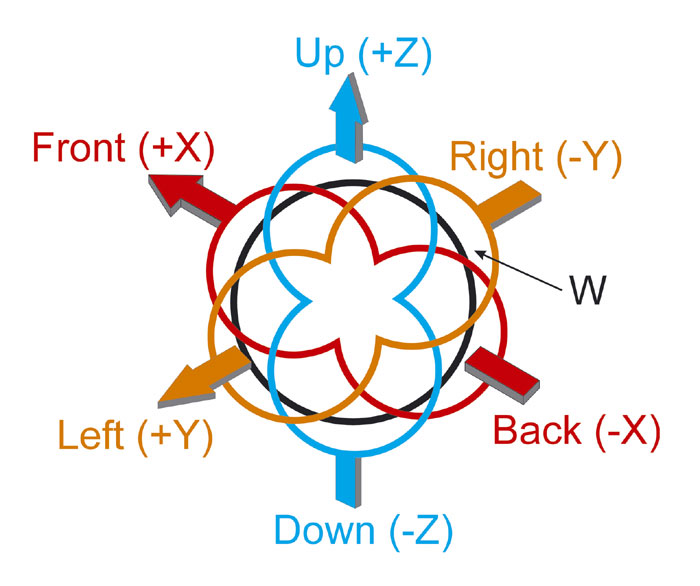
\includegraphics[scale = 0.3]{Sections/Background/images/soundFieldPolar.jpg}
				\end{minipage}
				\label{sfMic}
				\caption{\textbf{Left}: Picture of a Soundfield microphone with coincident capsules exposed \textbf{Right}: Soundfield microhpone polar pattern \cite{soundFieldMic}}
			\end{figure}

	\subsection{The Virtual Singing Studio}
		The \ac{VSS} is a loudspeaker based room acoustics simulator used as a tool for analysing the correlation between room acoustic characteristics and vocal performance parameters as part of Dr Jude Breretons PhD Thesis \cite{Brereton2014}.

		\subsubsection{How It Works}

		%RIR with ambisonics

		%Live audio input with RIR

		%Max patch and .spat


\subsubsection{Synthetic RIRs}

\paragraph{Geometrical Methods}

This is a method

\subsection{Ambisonics}



\end{document}